%!TEX program = xelatex
\documentclass[dvipsnames, svgnames,a4paper,11pt]{article}
% ----------------------------------------------------
%   中山大学物理与天文学院本科实验报告模板
%   作者:Huanyu Shi,2019级
%   知乎:https://www.zhihu.com/people/za-ran-zhu-fu-liu-xing
%   Github:https://github.com/huanyushi/SYSU-SPA-Labreport-Template
%   Last update : 2023.4.10
% ----------------------------------------------------

% ----------------------------------------------------- 
%	加边框的命令
%	参考:https://tex.stackexchange.com/questions/531559/how-to-add-the-page-border-for-first-two-pages-in-latex
\usepackage{tikz}
\usetikzlibrary{calc}
\usepackage{eso-pic}
\AddToShipoutPictureBG{%
\begin{tikzpicture}[overlay,remember picture]
\draw[line width=0.6pt] % 边框粗细
    ($ (current page.north west) + (0.6cm,-0.6cm) $)
    rectangle
    ($ (current page.south east) + (-0.6cm,0.6cm) $); % 边框位置
\end{tikzpicture}}


\usepackage{xcolor}
\definecolor{c1}{HTML}{2752C9} % 目录颜色
\definecolor{c2}{RGB}{190,20,83} % 引用颜色

\usepackage{ctex}
\usepackage[top=28mm,bottom=28mm,left=15mm,right=15mm]{geometry}
\usepackage{hyperref} 
\hypersetup{
	colorlinks,
	linktoc = section, % 超链接位置,选项有section, page, all
	linkcolor = c1, % linkcolor 目录颜色
	citecolor = c1  % citecolor 引用颜色
}
\usepackage{amsmath,enumerate,multirow,float}
\usepackage{tabularx}
\usepackage{tabu}
\usepackage{subfig}
\usepackage{fancyhdr}
\usepackage{graphicx}
\usepackage{wrapfig}  
\usepackage{physics}
\usepackage{appendix}
\usepackage{amsfonts}

%
\usepackage{tcolorbox}
\tcbuselibrary{skins,breakable}
\newtcolorbox{tbox}[2][]{
    colframe=black!70!,
    breakable,
    enhanced,
	boxrule =0.5pt,
    title = {#2},
    fonttitle = \large\kaishu\bfseries,
	drop fuzzy shadow,
    #1
}
\newtcolorbox[auto counter,number within=section]{question}[1][]{
  top=2pt,bottom=2pt,arc=1mm,
  boxrule=0.5pt,
%   frame hidden,
  breakable,
  enhanced, %跨页后不会显示下边框
  coltitle=c1!80!gray,
  colframe=c1,
  colback=c1!3!white,
  drop fuzzy shadow,
  title={思考题~\thetcbcounter:\quad},
  fonttitle=\bfseries,
  attach title to upper,
  #1
}

% ---------------------------------------------------------------------
%	利用cleveref改变引用格式,\cref是引用命令
\usepackage{cleveref}
\crefformat{figure}{#2{\textcolor{c2}{图 #1}}#3} % 图片的引用格式
\crefformat{equation}{#2{(\textcolor{c2}{#1})}#3} % 公式的引用格式
\crefformat{table}{#2{\textcolor{c2}{表 #1}}#3} % 表格的引用格式


% ---------------------------------------------------------------------
%	页眉页脚设置
\fancypagestyle{plain}{\pagestyle{fancy}}
\pagestyle{fancy}
\lhead{\kaishu 中山大学物理与天文学院基础物理实验\uppercase\expandafter{\romannumeral2}} % 左边页眉,学院 + 课程
\rhead{\kaishu  \quad 光学相差实验Ⅰ} % 右边页眉,实验报告标题
\cfoot{\thepage} % 页脚,中间添加页码


% ---------------------------------------------------------------------
%	对目录、章节标题的设置
\renewcommand{\contentsname}{\centerline{\huge 目录}}
\usepackage{titlesec}
\usepackage{titletoc}
% \titleformat{章节}[形状]{格式}{标题序号}{序号与标题间距}{标题前命令}[标题后命令]
\titleformat{\section}{\centering\LARGE\songti}{}{1em}{}

% ---------------------------------------------------------------------
%   listing代码环境设置
\usepackage{listings}
\lstloadlanguages{python}
\lstdefinestyle{pythonstyle}{
backgroundcolor=\color{gray!5},
language=python,
frameround=tftt,
frame=shadowbox, 
keepspaces=true,
breaklines,
columns=spaceflexible,                   
basicstyle=\ttfamily\small, % 基本文本设置,字体为teletype,大小为scriptsize
keywordstyle=[1]\color{c1}\bfseries, 
keywordstyle=[2]\color{Red!70!black},   
stringstyle=\color{Purple},       
showstringspaces=false,
commentstyle=\ttfamily\scriptsize\color{green!40!black},%注释文本设置,字体为sf,大小为smaller
tabsize=2,
morekeywords={as},
morekeywords=[2]{np, plt, sp},
numbers=left, % 代码行数
numberstyle=\it\tiny\color{gray}, % 代码行数的数字字体设置
stepnumber=1,
rulesepcolor=\color{gray!30!white}
}




% ---------------------------------------------------------------------
%	其他设置
\def\degree{${}^{\circ}$} % 角度
\graphicspath{{./images/}} % 插入图片的相对路径
\allowdisplaybreaks[4]  %允许公式跨页 % 导入模板的相关设置
\usepackage{lipsum}
\usepackage{enumitem}
%\setlist[enumerate]{label=\textup{(\arabic*)}}



%---------------------------------------------------------------------
%	正文
%---------------------------------------------------------------------

\begin{document}


\begin{table}
	\renewcommand\arraystretch{1.7}
	\begin{tabularx}{\textwidth}{
			|X|X|X|X
			|X|X|X|X|}
		\hline
		\multicolumn{2}{|c|}{预习报告}&\multicolumn{2}{|c|}{实验记录}&\multicolumn{2}{|c|}{分析讨论}&\multicolumn{2}{|c|}{总成绩}\\
		\hline
		\LARGE25 & & \LARGE30 & & \LARGE25 & & \LARGE80 & \\
		\hline
	\end{tabularx}
\end{table}


\begin{table}
	\renewcommand\arraystretch{1.7}
	\begin{tabularx}{\textwidth}{|X|X|X|X|}
	\hline
	年纪、专业:& 物理学 & 组号:& 实验班2\\
	\hline
	姓名:& 戴鹏辉  & 学号: & 2344016 \\
	\hline
	时间:& 2024/03/05 & 教师签名:& \\
	\hline
	\end{tabularx}
\end{table}

\begin{center}
	\LARGE CA3 \quad 原子的发射和吸收光谱观测分析实验
\end{center}

\textbf{【实验报告注意事项】}
\begin{enumerate}
	\item 实验报告由三部分组成:
	\begin{enumerate}[label=\textup{(\arabic*)}]
		\item 预习报告:课前认真研读\underline{\textbf{实验讲义}},实验所需的仪器设备、用具及其使用、完成课前预习思考题;了解实验需要测量的物理量,并根据要求提前准备实验记录表格(可以参考实验报告模板,可以打印)。\textcolor{red}{\textbf{(25分)}}
		
	    \item 实验记录:认真、客观记录实验条件、实验过程中的现象以及数据。实验记录请用珠笔或者钢笔书写并签名(\textcolor{red}{\textbf{用铅笔记录的被认为无效}})。\textcolor{red}{\textbf{保持原始记录,包括写错删除部分,如因误记需要修改记录,必须按规范修改。}}(不得输入电脑打印,但可扫描手记后打印扫描件);离开前请实验教师检查记录并签名。\textcolor{red}{\textbf{(30分)}}
	    
	    \item 数据处理及分析讨论:处理实验原始数据(学习仪器使用类型的实验除外),对数据的可靠性和合理性进行分析;按规范呈现数据和结果(图、表),包括数据、图表按顺序编号及其引用;分析物理现象(含回答实验思考题,写出问题思考过程,必要时按规范引用数据);最后得出结论。\textcolor{red}{\textbf{(25分)}}
	    
	\end{enumerate}
	\textbf{实验报告就是将预习报告、实验记录、和数据处理与分析合起来,加上本页封面。}
	\item 每次完成实验后的一周内交\textbf{实验报告}(特殊情况不能超过两周)。
	\item 注意事项:
		\begin{enumerate}[label=\textup{(\arabic*)}]
			\item 实验中\textcolor{red}{\textbf{光纤不能过度弯折}};
			\item 信号强度不能过饱和值;
			\item 光源长时间通电后会\textcolor{red}{\textbf{发热}},小心烫手,切换光源时务必注意(可等断电冷却后再碰);
			\item \textcolor{red}{\textbf{请提前了解光纤光谱仪的基本工作原理与关键参数等。}}
		
		

		\end{enumerate}
\end{enumerate}



\clearpage
\tableofcontents
\clearpage

\setcounter{section}{0}
\section{CA3 \quad 原子的发射和吸收光谱观测分析实验 \quad\heiti 预习报告}
	
\subsection{实验目的}
	\begin{enumerate}
		\item 原子发射光谱的观测:
			\begin{enumerate}
				\item 学习光纤光谱仪的使用;
				\item 观测钠原子光谱,了解碱金属原子光谱的一般规律;
				\item 观测汞原子光谱,了解中外层电子与原子核相互作用;
				\item 观测多种光源的发射光谱,了解线光谱与连续谱的异同。
			\end{enumerate}
		\item  原子吸收光谱的观测:
			\begin{enumerate}
				\item 调配不同浓度的高锰酸钾水溶液;
				\item 测量高锰酸钾水溶液的紫外-可见吸收光谱,找出吸收峰;
				\item 测量不同浓度高锰酸钾水溶液的紫外-可见吸收光谱,验证比尔定律;
				\item 测量不同片数玻璃基板的透过光谱,验证朗伯定律。
			\end{enumerate}
	\end{enumerate}
	

\subsection{仪器用具}
	\begin{table}[htbp]
		\centering
		\renewcommand\arraystretch{1.6}
		% \setlength{\tabcolsep}{10mm}
		\begin{tabular}{p{0.05\textwidth}|p{0.20\textwidth}|p{0.05\textwidth}|p{0.5\textwidth}}
		\hline
		编号& 仪器用具名称 & 数量 &  主要参数(型号,测量范围,测量精度等) \\
		\hline
		1 & 多种光源 	& 若干	& {\footnotesize 低压汞灯、低压钠灯、氢氘灯、 溴钨灯、多种颜色的发光二极管} \\
	
		2 & 滤光片 	& 2 	& 白片、红片 \\
		
		3 & 测控计算机 & 1 &  \\
		
		4 & 光谱观测和分析仪器 & 1 & 光纤光谱仪\\
		
		5 & 高锰酸钾水溶液 & -- &  \\
		
		6 & 玻璃基板 & 1  &  \\
		
		7 & 比色皿 & 1 & \\
		
		\hline
		\end{tabular}
	\end{table}

\subsection{原理概述}

		\begin{enumerate}
		\item 原子发射光谱的观测:
			\begin{enumerate}
				\item \textbf{碱金属原子光谱}:\\
					碱金属和氢原子一样,核外只有一个价电子,但在碱金属原子中除了一个价电子外,还有封闭在内的壳层电子,这些内封闭的电子和原子核统称为原子实。当价电子贯穿原子实时,会产生异于氢原子光谱的一系列特点。碱金属原子光谱线公式为:
					\[
					\widetilde{v}=R(\frac{1}{n_2^{*2}}-\frac{1}{n_1^{*2}})=\frac{R}{{(n'-{\mu'}_{l'})}^2}-\frac{R}{{(n-\mu_l)}^2}
					\]
					其中,$\widetilde{v}$为光谱线的波数; $R$ 为里德堡常数;$n'$与$n$分别为始态和终态的主量子数;$n_2^{*}$与$n_1^{*}$分别为始态和终态的有效量子数;$l′$与$l$分别为该量子数决定之能级的轨道量子数;$𝜇{\mu'}_{l'}$与$\mu_l$分别为始态和终态的量子缺(也称量子改正数,量子亏损)。
					
					以钠原子为例来说,它的光谱分四个线系:主线系、锐线系、漫线系、基线系。对于某一线系谱线的波数公式可写为:
					\[\tilde{\nu} = A_{n'l'}-\dfrac{R}{(n-\mu_{l})^2}\]
					
					从钠原子光谱中,可以看出各个线系的一些明显特征,这些特征也为其它碱金属原子光谱所具有。
					\textbf{各线系的共同特点是}:
						\begin{enumerate}
							\item 同一线系内,随着波长减小(即向短波方向),相邻谱线的波数差逐渐减小,最终趋于一个极限,即连续谱与分立谱的边界。这是由于能级愈高,能级间的距离愈小,最终能级间的差别变得模糊。
							
							\item 在同一线系内,随着波长减小,谱线的强度逐渐减小。这是因为能级愈高,将原子从基态激发到该状态的能量也愈大,因此愈向短波方向,激发原子的难度愈大。
						\end{enumerate}
					\textbf{各线系的区别}:
						\begin{enumerate}
							\item 各线系所在的光谱区域不同。主线系的谱线大部分在紫外区,只有双黄线(钠的主共振线)在可见光区。锐线系和漫线系的谱线大部分在可见光区,基线系的谱线则在红外区。
							
							\item s 能级是单重的,p、d、f 能级是双重的。主线系和锐线系的谱线是双线的,漫线系和基线系的谱线是复双重线的。主线系的双线是由于3s能级与3p、4p等能级间的阶跃产生的,锐线系的双线则是内3p能级与各s能级之间的跃迁产生的。
							
							\item 从谱线的外观上看,主线系的谱线强度较大,锐线系的谱线轮廓清晰,漫线系的谱线显得弥漫,一般复双重线连成一片。
						\end{enumerate}
						
				\item \textbf{单色仪色散系统}:\\
					单色仪是一种用于分离和选择特定波长光线的光学仪器,其色散系统可以分为棱镜单色仪和光栅单色仪两种类型。棱镜单色仪使用棱镜作为色散元件,通过折射不同波长光线的角度差异实现色散。而光栅单色仪则使用光栅作为色散元件,利用光栅的周期性结构引起光的衍射,不同波长的光线经过衍射后呈现不同的衍射角度,从而实现色散。通过调整色散元件的位置或角度,单色仪可以选择性地分离和选择特定波长的光线,最终产生单色光用于实验或分析。
				
				\item \textbf{光谱仪和光学多通道分析仪}:\\
					光谱仪是一种用于记录光线的波长和强度分布的仪器,它包括棱镜光谱仪和光栅光谱仪两种类型。光谱仪的工作原理是利用棱镜或光栅将入射光线按波长分散成不同的光束,然后利用光电倍增管、CCD或CMOS传感器等设备记录这些光束,形成光谱图像。光学多通道分析仪是一种光谱仪的变体,它包括光栅单色仪、CCD或CMOS接收单元、扫描系统、电子放大器、A/D采集单元和计算机等组件。光学多通道分析仪通过这些组件实现对光谱的高效捕获和分析,具有高分辨率和精确度的特点。
					
					\begin{figure}[htbp]
						\centering
						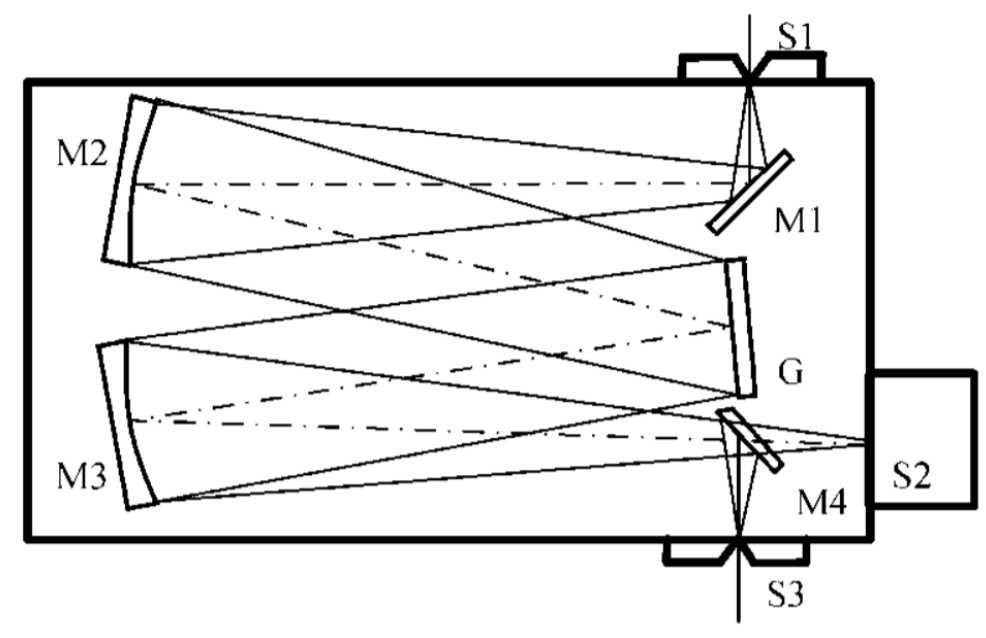
\includegraphics[width=0.4\textwidth]{graph1.png}
						\caption{光学多通道分析仪原理示意图}
						\label{fig:graph1}
					\end{figure}
					
			\end{enumerate}
			
			
			
		\item \textbf{原子吸收光谱的观测}:
			\begin{enumerate}
				\item \textbf{光的吸收}:
					
					在吸收过程中,物质的原子或分子吸收了入射的辐射能,从基态跃迁至高能级的激发态,吸收的能量与电磁辐射的频率成正比,符合普朗克公式:
					\[ E = h\nu \]
					光的吸收是指光波穿过介质后光强减弱的现象。除了真空外,几乎所有介质对电磁波都不完全透明,都会发生吸收。根据吸收特性,吸收可分为一般吸收和选择吸收。一般吸收是指在一定波长范围内,物质对光的吸收不随波长变化;选择吸收则是指吸收随波长变化的现象。物质分子的能级结构决定了其吸收电磁辐射的能力,能级间的能量差越大,吸收越小,形成了一般吸收和选择吸收的特性。吸收分光光度法利用物质分子对电磁辐射的选择吸收特性,用于测量物质的吸收光谱,从而进行分析和研究。
				\item \textbf{朗伯定律}:\\
					朗伯定律(Lambert's law)是描述光线透过吸收性均匀介质时光强衰减规律的基本定律。朗伯定律的数学表示式为:
					\[ I = I_0 e^{-kl} \]
					吸收系数$k$是波长的函数,在一般吸收的波段内, $k$ 值很小,并且近乎于一常数;在选择吸收波段内, $k$ 值甚大,并且随波长的不同而有显著的变化。
					
					\begin{figure}[htbp]
						\centering
						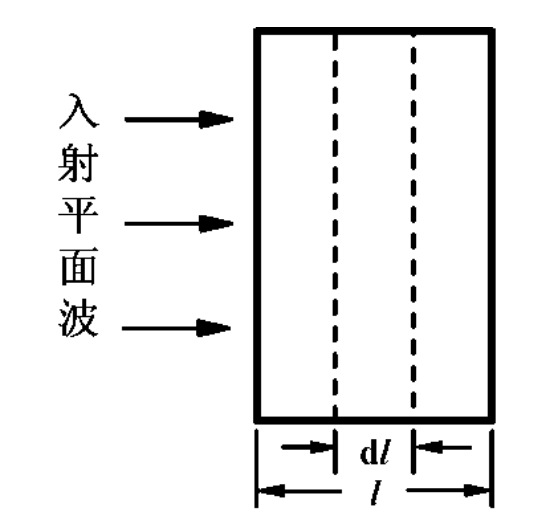
\includegraphics[width=0.2\textwidth]{graph6.png}
						\caption{均匀媒质对光的吸收}
						\label{fig:graph6}
					\end{figure}
					
				\item \textbf{比尔定律}:\\
					比尔定律(Beer's law),也称为比尔-朗伯定律(Beer-Lambert law),是描述光线透过吸收性均匀介质时光强衰减规律的定律,是朗伯定律的一个特例。比尔定律的数学形式为:
					\[ A = \alpha c l \]
					$A$表示吸光度,$\alpha$是摩尔吸光系数,$c$为浓度,$l$是光通过溶液的路径长度。
					在比尔定律成立时,就可用测量吸收的方法来测定物质的浓度。这就是快速测定物质浓度的吸收光谱分析法。
					
					\begin{figure}[htbp]
						\centering
						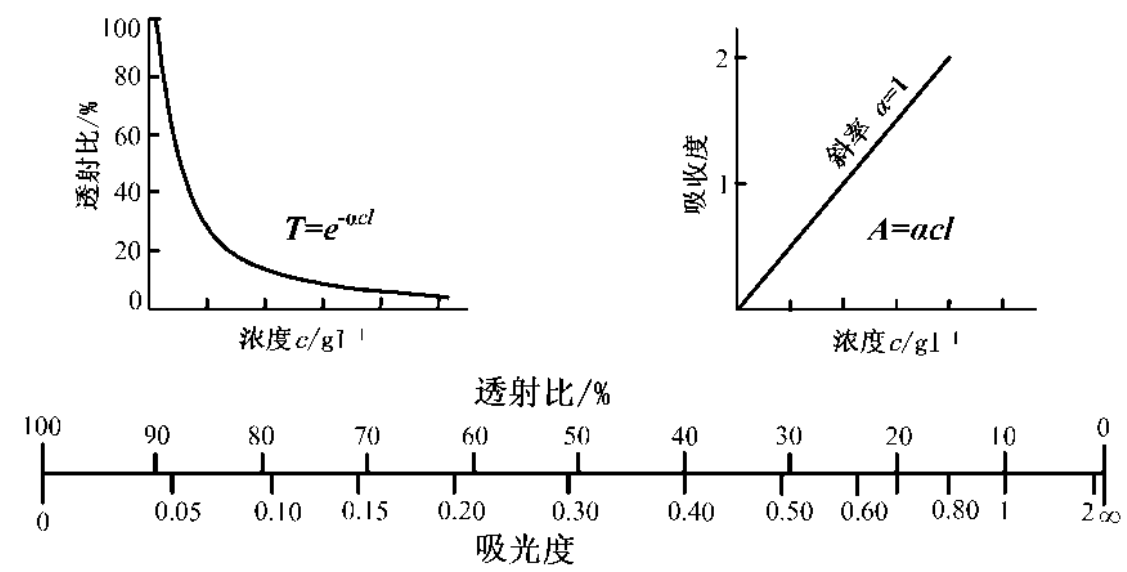
\includegraphics[width=0.6\textwidth]{graph7.png}
						\caption{比尔定律示意图和吸收度、投射比标度的比较}
						\label{fig:graph7}
					\end{figure}
%				\item 光谱仪和光学多通道分析仪:
					
				
			\end{enumerate}
		
	\end{enumerate}


\subsection{实验前思考题}
	%思考题1
	\begin{question}
		日常生活中,光源可以分为热光源和冷光源,请分别说明太阳光、蜡烛、白炽灯、荧光灯、 LED 灯等属于哪一类光源,为什么?
	\end{question}
	
	在日常生活中,光源可以分为热光源和冷光源两类,它们的区别在于发光原理不同。
	\begin{enumerate}
		\item 热光源:热光源的发光原理是物体受热后发出的光。典型的热光源包括太阳光和白炽灯。太阳光是地球主要的光源,它的光谱是连续的,包含了可见光、紫外线和红外线等各种波长的光。白炽灯的发光原理是通电后灯丝受热发光,因此也属于热光源。
		
		\item 冷光源:冷光源的发光原理是物质受激发后发出的光。典型的冷光源包括蜡烛、荧光灯和LED灯。蜡烛的燃烧产生火焰,火焰中的碳颗粒被激发后发出光,因此属于冷光源。荧光灯通过电流激发荧光粉发光,LED灯则是通过半导体材料电子跃迁产生光,它们都属于冷光源。
	\end{enumerate}
	
	综上所述,太阳光和白炽灯属于热光源,而蜡烛、荧光灯和LED灯属于冷光源。

	%思考题2
%	\begin{question}
%		XXXXXXXXXXXXXXXXXXXXXXX
%	\end{question}
	

\clearpage
\begin{table}
	\renewcommand\arraystretch{1.7}
	\centering
	\begin{tabularx}{\textwidth}{|X|X|X|X|}
	\hline
	专业:& 物理学 &年级:& 2022级 \\
	\hline
	姓名:& 戴鹏辉 & 学号:& 22344016 \\
	\hline
	室温:& 26℃ & 实验地点: & A501 \\
	\hline
	学生签名:& & 评分: &\\
	\hline
	实验时间:& 2024/03/07 & 教师签名:&\\
	\hline
	\end{tabularx}
\end{table}

\section{CA3 \quad 原子的发射和吸收光谱观测分析实验 \quad\heiti 实验记录}
\subsection{实验内容和步骤}

	\subsubsection{实验一 \quad 原子发射光谱的观测}
		
		\begin{enumerate}
			\item 拍摄钠灯光谱
				\begin{enumerate}
					\item 选择合适的积分次数和积分时间。实际实验中选择了“积分时间2ms,积分次数100次”
					
					\item 将光纤一端连接光谱仪,一端关闭,测量暗噪声。 
					
					\item 将光纤另一端装上支架,将支架对准环境,测量环境噪声。
					
					\item 将暗噪声与环境噪声都扣除后,将支架对准钠灯,测量钠灯光谱。
					
				\end{enumerate}
				
				得到的钠灯光谱如下图所示:
				
				\begin{figure}[htbp]
					\centering
					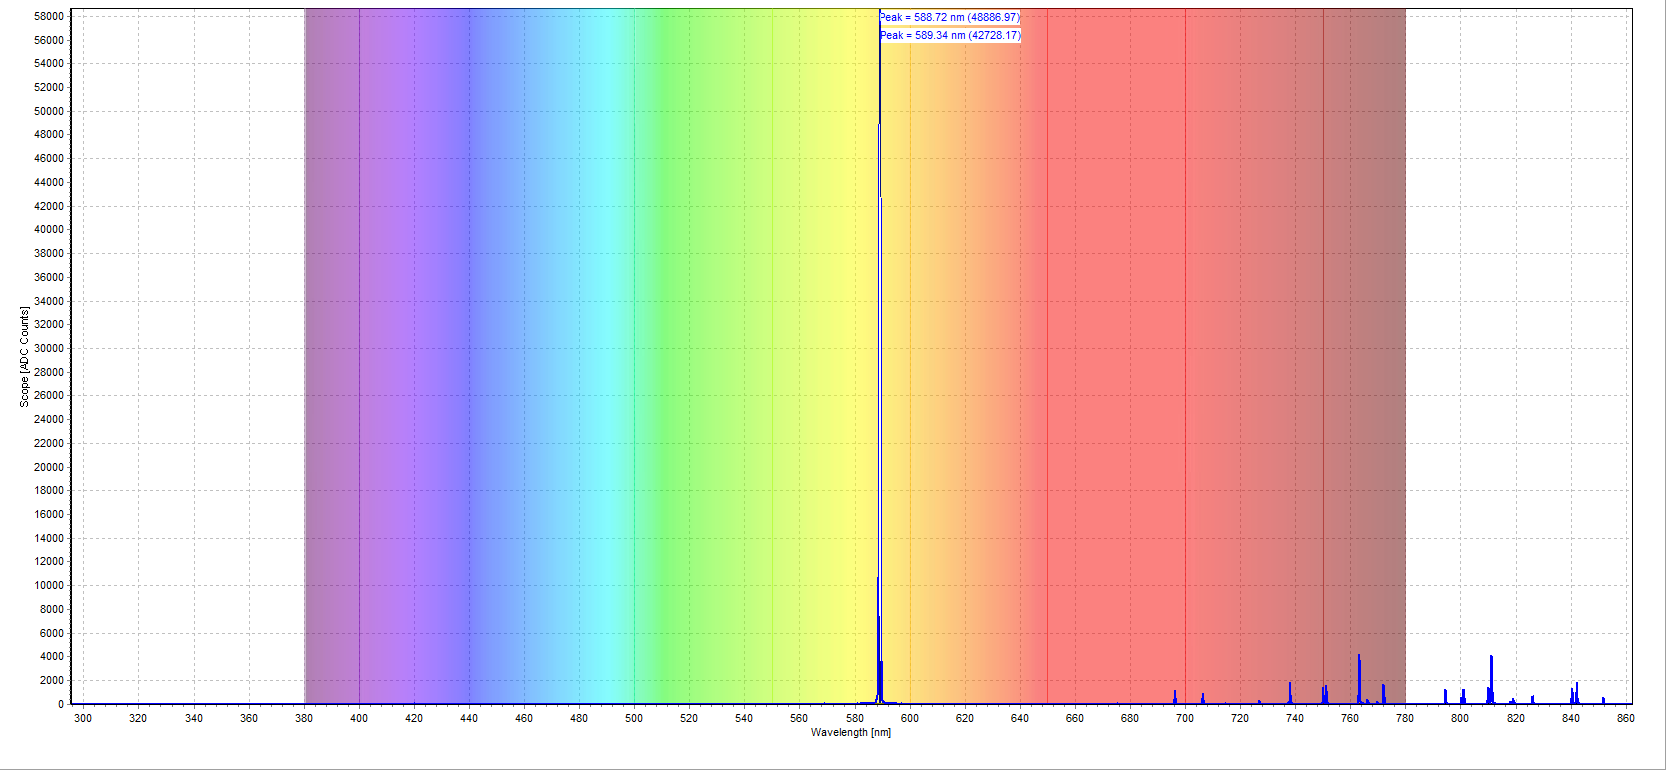
\includegraphics[width=1\textwidth]{Na2.png}
					\caption{钠灯光谱}
					\label{fig:Na2}
				\end{figure}
				
				\begin{figure}[htbp]
					\centering
					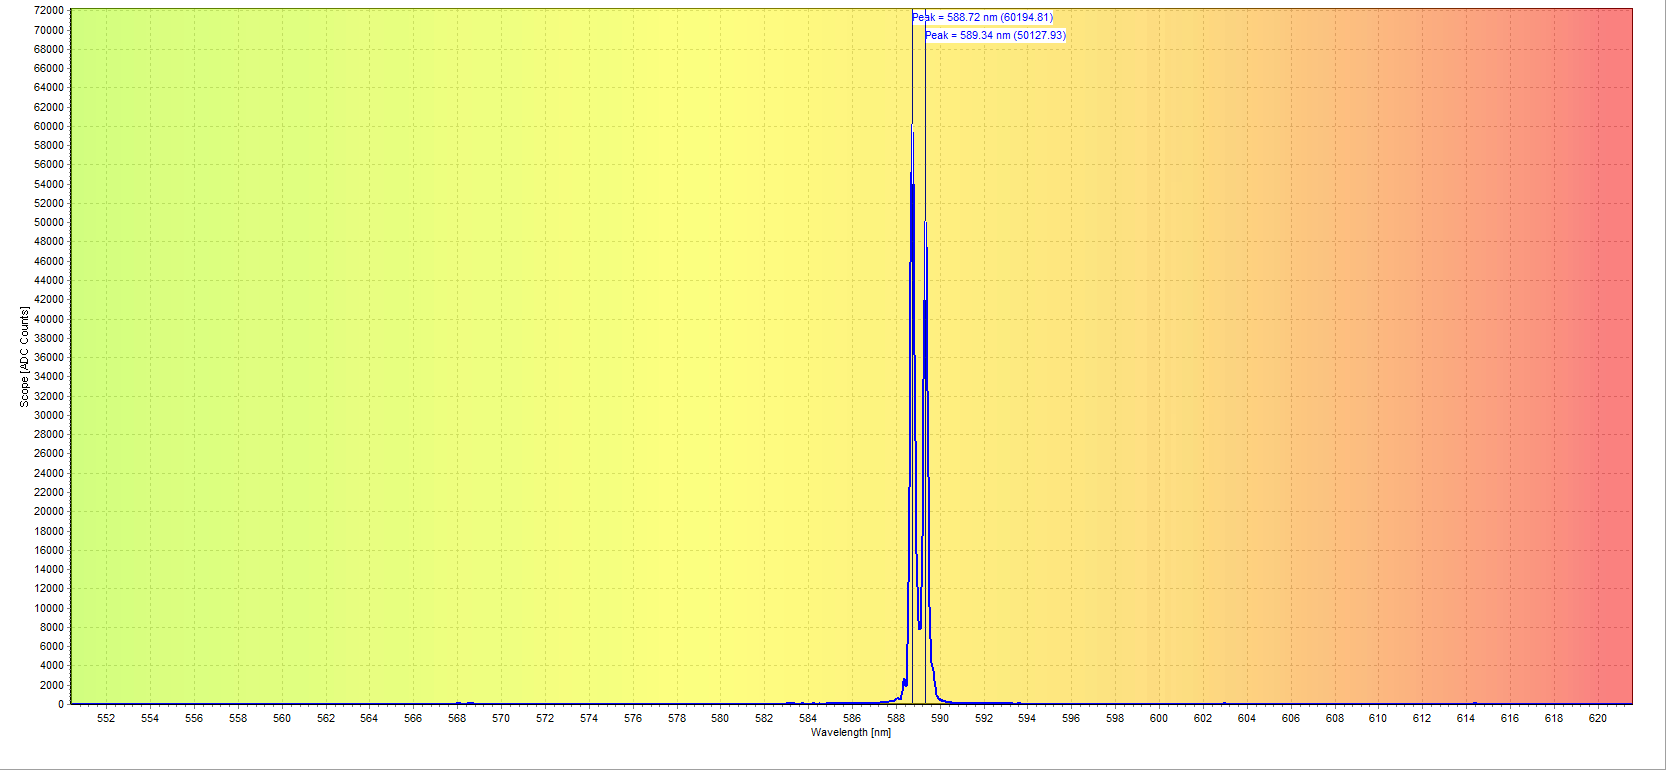
\includegraphics[width=1\textwidth]{Na2-589.png}
					\caption{钠灯光谱双黄线}
					\label{fig:Na2-589}
				\end{figure}
				
			\item 拍摄汞灯光谱
			
				重复上述步骤,测量暗噪声和环境噪声。将暗噪声与环境噪声都扣除后,将支架对准汞灯,测量汞灯光谱。
				
				
				得到的汞灯光谱如下图所示:
				
				\begin{figure}[htbp]
					\centering
					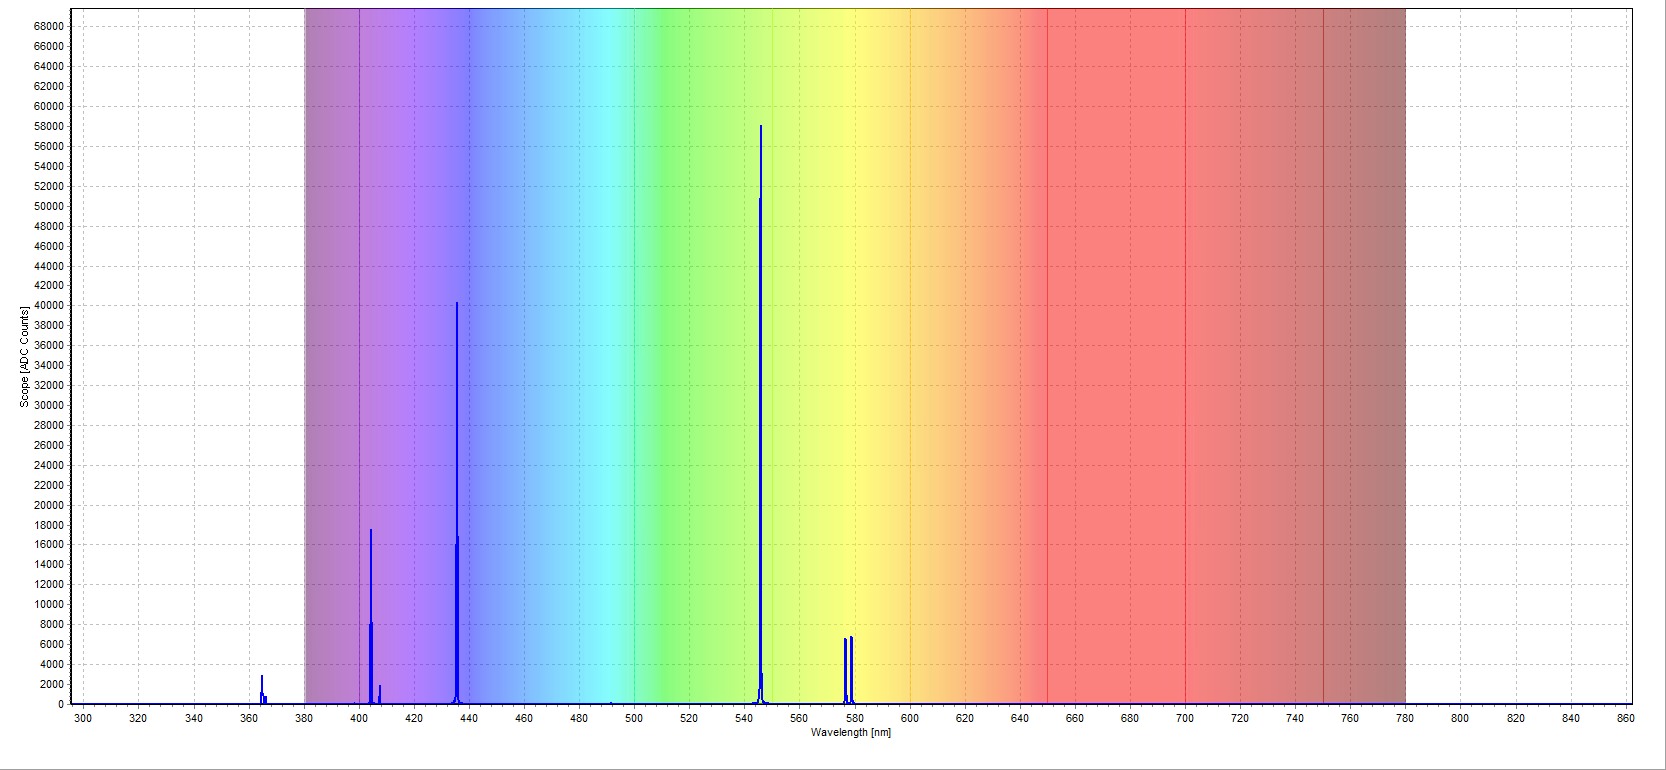
\includegraphics[width=1\textwidth]{Hg1.png}
					\caption{汞灯光谱}
					\label{fig:Hg1}
				\end{figure}
				
				\begin{figure}[htbp]
					\centering
					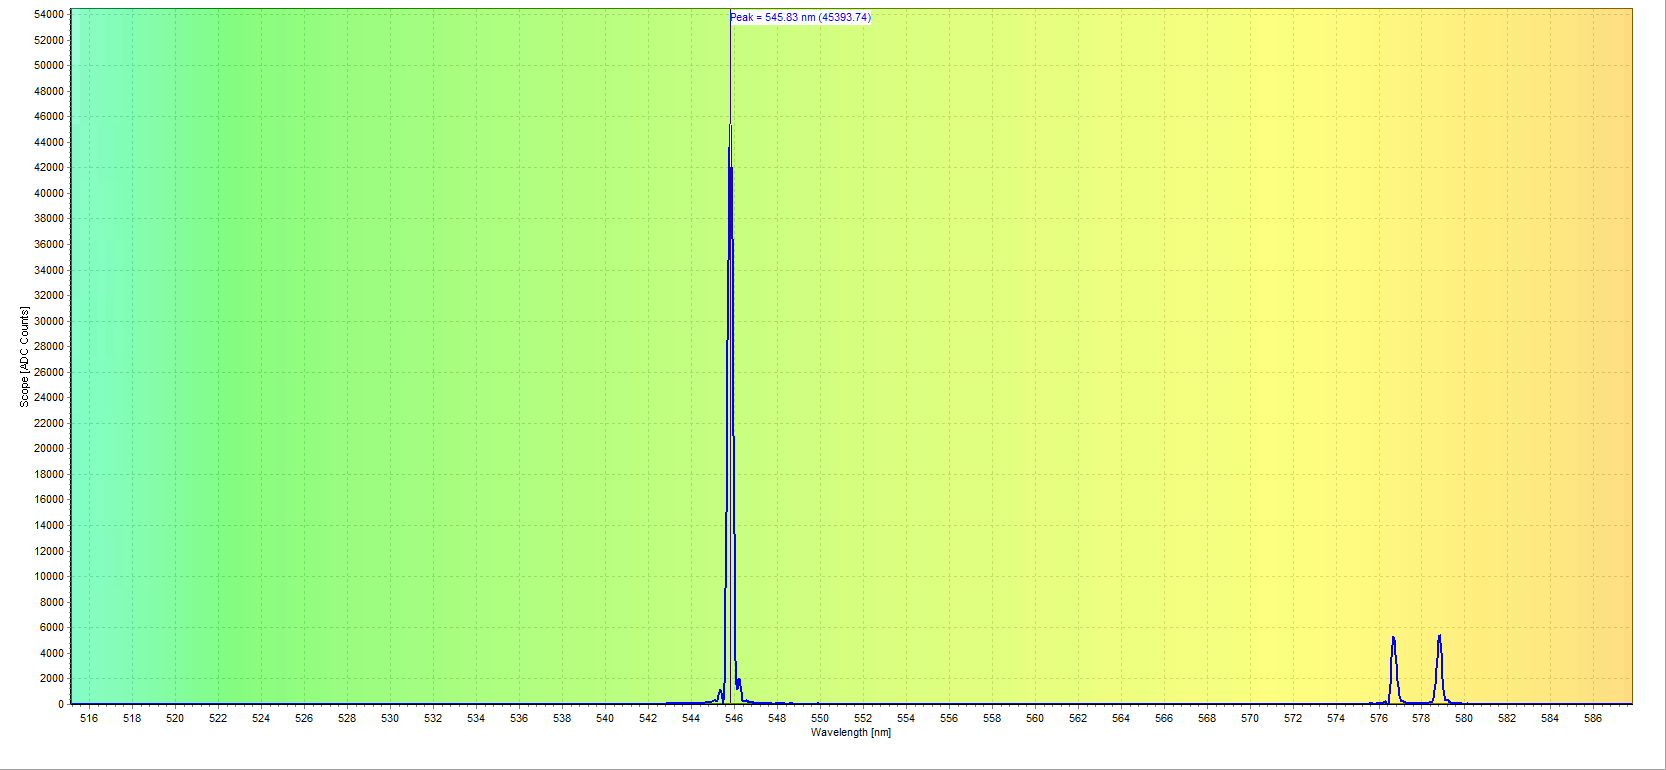
\includegraphics[width=1\textwidth]{Hg2-546nm.png}
					\caption{汞灯光谱峰值}
					\label{fig:Hg2-546}
				\end{figure}
				
			\item 拍摄手机屏幕光谱
			
				重复上述步骤,测量暗噪声和环境噪声。将暗噪声与环境噪声都扣除后,将支架对准手机屏幕,测量手机屏幕光谱。其中手机显示全白画面。
				
				得到的手机屏幕光谱如下图所示:
				
				\begin{figure}[htbp]
					\centering
					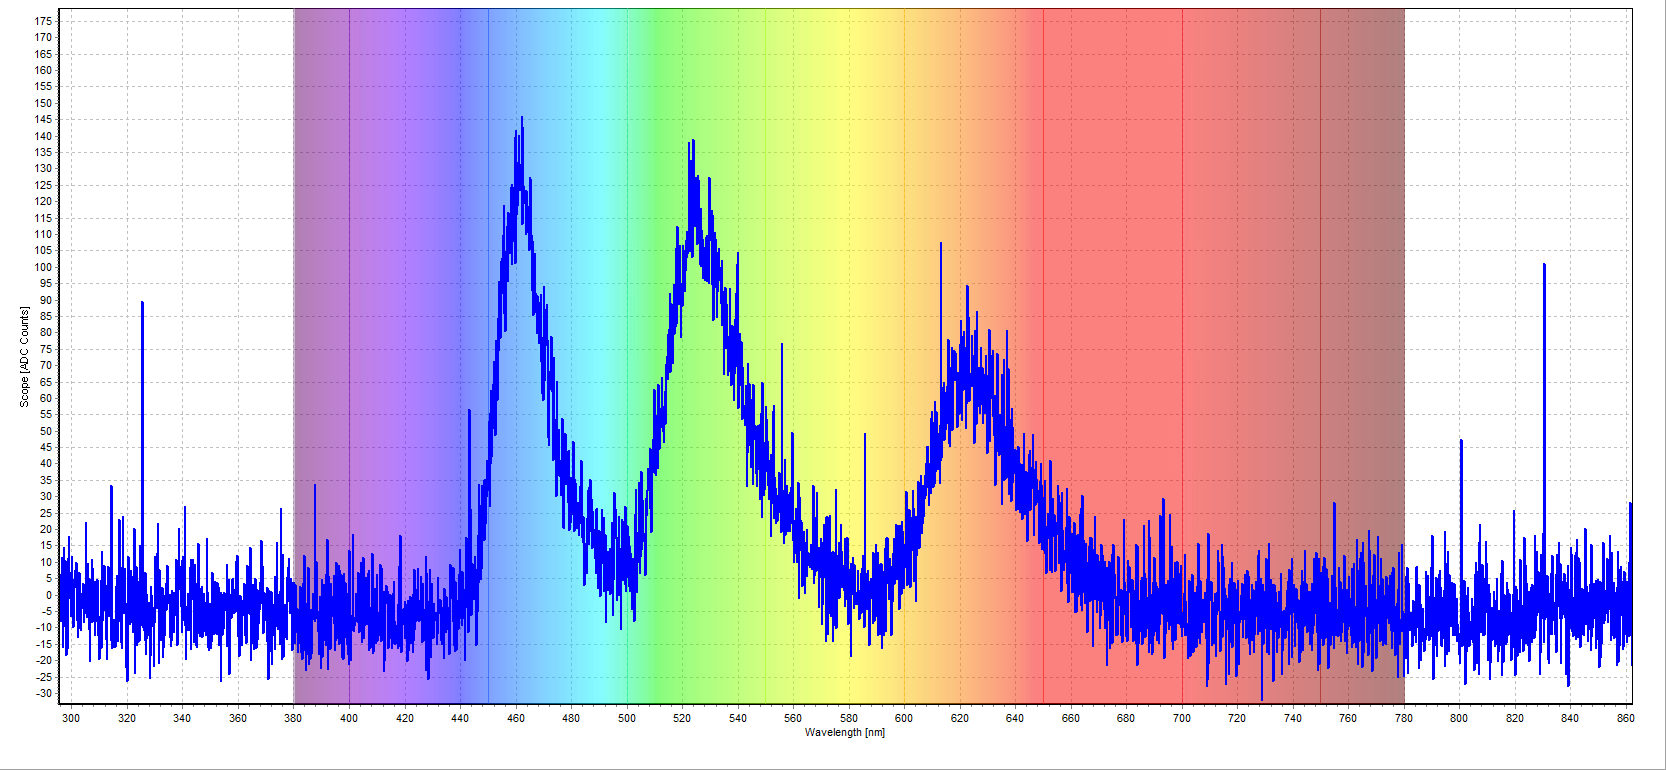
\includegraphics[width=1\textwidth]{phone.png}
					\caption{手机屏幕光谱}
					\label{fig:phone}
				\end{figure}
		\end{enumerate}
		
		
		
	

	\subsubsection{实验二 \quad 原子吸收光谱的观测}

		

%	\subsubsection{实验三 \quad 拍摄手机屏幕光谱}
	
	


%\subsection{实验数据记录}



%\subsection{原始数据记录}



\subsection{实验过程中遇到的问题记录}

\begin{enumerate}
	\item 	
	
	\item 	
	
	\item 	
	
	\item 	
	
	\item 	
	
\end{enumerate}
	

\clearpage
\begin{table}
	\renewcommand\arraystretch{1.7}
	\begin{tabularx}{\textwidth}{|X|X|X|X|}
	\hline
	专业:& 物理学 &年级:& 2022级\\
	\hline
	姓名: & 戴鹏辉 & 学号:& 22344016\\
	\hline
    日期:& 2024/xx/xx & 评分: &\\
	\hline
	\end{tabularx}
\end{table}

\section{CA3 \quad 原子的发射和吸收光谱观测分析实验 \quad\heiti 分析与讨论}

\subsection{实验数据分析}

	\subsubsection{实验一 测量光栅常数}
		由表1中的数据,可计算得到各级衍射条纹的衍射角,如下表所示
		
		\begin{center}
			\begin{tabular}{|c|c|c|c|}
				\hline
				$\varphi_{+1}$ & $\varphi_{+2}$ & $\varphi_{-1}$ & $\varphi_{-2}$ \\
				\hline
				10°09′ & 20°37′ & 10°10′ & 20°47′ \\
				\hline
			\end{tabular}
		\end{center}

		
		则可由正负级衍射角计算平均值,并根据光栅衍射公式$k\lambda=d\sin{\varphi}$,计算光栅常数,其中钠灯的谱线已知,取$\lambda=589.4nm$,则计算结果如下表所示
		
		\begin{center}
			\begin{tabular}{|c|c|c|}
				\hline
				$\varphi_1$ & $\varphi_2$ &  \\
				\hline
				10°09′ & 20°42′ &  \\
				\hline
				$d_1$ & $d_2$ & $\overline{d}$ \\
				\hline
				$3.344\times{10}^{-6}m$ & $3.334\times{10}^{-6}m$ & $3.339\times{10}^{-6}m$ \\
				\hline
			\end{tabular}
		\end{center}

		下面计算不确定度:
		
		\begin{enumerate}
			\item  角度的重复测量引起的标准不确定度分量$u_1$,
					\[ u_1=\sqrt{\sum{(\left|\frac{\partial d}{\partial\varphi_i}\right|\sigma_i)}^2}=4.55\times{10}^{-8}m \]
					
			\item  仪器的示值误差引起的标准不确定度分量$u_2$,由分光计游标最小分度值1’,按照均匀分布考虑
					\[ u_2=\sqrt{\sum{(\left|\frac{\partial d}{\partial\varphi_i}\right|\sigma_i)}^2}=1.99\times{10}^{-7}m \]
			
			\item  合成不确定度
					\[ u_c=\sqrt{\sum{(u_i)}^2}=2.04\times{10}^{-7}m \]
			
			\item 展伸不确定度\\
					考虑正态分布,取置信概率为95\%,查表得包含因子$k=1.96$
					
					则最终测量结果表示为 $ d=\bar{d}\pm ku_c=(3.34\pm0.40)\times{10}^{-6}m$
					
					
		\end{enumerate}
		
		分析误差来源
			\begin{enumerate}
				\item 可能是由于光栅本身的刻线不均匀,或者刻线与仪器转轴不平行,导致不同级次之间的测量数据计算所得结果之间有较大误差;这是仪器本身的系统误差,无法消除,只能通过更换质量更好的光栅来避免。
				
				\item 平行光管进光狭缝的宽度可能过宽,使得入射谱线的宽度也变宽,则会降低谱线的分辨率和对比度,使得测量衍射角时不准确,从而影响计算结果。
			\end{enumerate}
		
		
		\subsubsection{实验二 测定未知光波波长及角色散率D}
			
			根据表2数据,重复实验一中的处理操作,计算正负级衍射角,计算平均值,并根据光栅衍射公式$k\lambda=d\sin{\varphi}$,计算不同衍射谱线对应光波波长,式中光栅常数取实验一中的计算结果 $d=3.34\times{10}^{-6}m$ ,则计算结果如下表所示
			
			\begin{center}
				\begin{tabular}{|c|c|c|c|}
					\hline
					\textbf{颜色} & \textbf{蓝色(b)} & \textbf{绿色(g)} & \textbf{黄色(y)} \\
					\hline
					$\varphi_{+1}$ & 07°29′ & 09°22′ & 09°58′ \\
					$\varphi_{+2}$ & 15°07′ & 19°02′ & 20°11′ \\
					$\varphi_{-1}$ & 07°32′ & 09°29′ & 10°00′ \\
					$\varphi_{-2}$ & 15°12′ & 19°10′ & 20°23′ \\
					\hline
					&  &  &  \\
					\hline
					$\varphi_1$ & 07°30′ & 09°25′ & 09°59′ \\
					$\varphi_2$ & 15°10′ & 19°06′ & 20°17′ \\
					\hline
					&  &  &  \\
					\hline
					$\lambda_1$ & 435.83nm & 546.30nm & 578.86nm \\
					$\lambda_2$ & 436.79nm & 546.29nm & 578.75nm \\
					$\overline{\lambda}$ & 436.31nm & 546.30nm & 578.80nm \\
					\hline
				\end{tabular}
			\end{center}

			下面计算不确定度:
				
			\begin{enumerate}
					\item 	角度的重复测量引起的标准不确定度分量$u_1$,
							\[ u_{b1}=\sqrt{\sum\left(\left|\frac{\partial\lambda}{\partial\varphi_i}\right|\sigma_i\right)^2}=0.402nm \]
							\[ u_{g1}=\sqrt{\sum\left(\left|\frac{\partial\lambda}{\partial\varphi_i}\right|\sigma_i\right)^2}=1.14nm \]
							\[ u_{y1}=\sqrt{\sum{(\left|\frac{\partial\lambda}{\partial\varphi_i}\right|\sigma_i)}^2}=1.36nm \]
					
					\item 仪器的示值误差引起的标准不确定度分量$u_2$,\\
							由分光计游标最小分度值1’,按照均匀分布考虑
							\[ u_{b2}=\sqrt{\sum{(\left|\frac{\partial\lambda}{\partial\varphi_i}\right|\sigma_i)}^2}=0.10nm \]
							\[ u_{g2}=\sqrt{\sum\left(\left|\frac{\partial\lambda}{\partial\varphi_i}\right|\sigma_i\right)^2}=0.13nm \]
							\[ u_{y2}=\sqrt{\sum{(\left|\frac{\partial\lambda}{\partial\varphi_i}\right|\sigma_i)}^2}=0.14nm \]
					
					\item 合成不确定度
							\[ u_{cb}=\sqrt{\sum{(u_i)}^2}=0.41nm  \quad u_{cg}=\sqrt{\sum\left(u_i\right)^2}=1.15nm  \quad u_{cy}=\sqrt{\sum{(u_i)}^2}=1.36nm \]
					
					\item 展伸不确定度
							考虑正态分布,取置信概率为95\%,查表得包含因子$k=1.96$ \\
							则最终测量结果表示为
							\[ \lambda_b=(436.31\pm0.41)nm  \quad \lambda_g=\left(546.30\pm1.15\right)nm \quad  \lambda_y=(578.80\pm1.36)nm \]
					
				\end{enumerate}
		
			将各谱线波长计算值与标准值比较(预习报告中所查得的数据),计算各谱线波长的相对误差(计算黄光谱线相对误差时,参考值取两条黄色谱线的平均波长),得到
			\[ \eta_b=\left|\frac{435.8-436.31}{435.8}\right|\times100\%=0.117\% \]
			\[ \eta_g=\left|\frac{546.1-546.30}{546.1}\right|\times100\%=0.037\% \]
			\[ \eta_y=\left|\frac{578.05-578.80}{578.05}\right|\times100\%=0.130\% \]
			
			下面计算角色散率,根据角色散率公式$D=\frac{d\theta}{d\lambda}=\frac{k}{d\cos{\theta}}$,由上表数据计算得
			
				\begin{center}
					\begin{tabular}{|c|c|c|c|}
						\hline
						\textbf{颜色} & \textbf{蓝色} & \textbf{绿色} & \textbf{黄色} \\
						\hline
						D1 & $2.98\times 10^{5} m^{-1}$ & $2.99\times 10^{5} m^{-1}$ & $3.00\times 10^{5} m^{-1}$ \\
						D2 & $6.11\times 10^{5} m^{-1}$ & $6.24\times 10^{5} m^{-1}$ & $6.29\times 10^{5} m^{-1}$ \\
						\hline
					\end{tabular}
				\end{center}


			
			下面计算角色散率的不确定度,重复上面的操作,最终包含不确定度结果如下表所示
			
			\begin{center}
				\begin{tabular}{|c|c|c|c|}
					\hline
					\textbf{颜色} & \textbf{蓝色} & \textbf{绿色} & \textbf{黄色} \\
					\hline
					D1 & $2.98 \pm 0.002 \times 10^{5} m^{-1}$ & $2.99 \pm 0.03 \times 10^{5} m^{-1}$ & $3.00 \pm 0.01 \times 10^{5} m^{-1}$ \\
					D2 & $6.11 \pm 0.07 \times 10^{5} m^{-1}$ & $6.24 \pm 0.004 \times 10^{5} m^{-1}$ & $6.29 \pm 0.10 \times 10^{5} m^{-1}$ \\
					\hline
				\end{tabular}
			\end{center}
			
			分析误差来源:
			
			\begin{enumerate}
				\item 			观察数据可发现,在测量2级谱线时,正负级衍射角的差偏大,个别数据甚至超过了10’(由于超过10’的数据是最后一组测量数据,故没有及时发现),说明光栅并未完全与平行光管光轴垂直,存在一个小角度偏差,引入了一定的系统误差。
				\item 			平行光管进光狭缝的宽度可能过宽,使得入射谱线的宽度也变宽,则会降低谱线的分辨率和对比度,使得测量衍射角时不准确,从而影响计算结果。
			\end{enumerate}
			
			
\subsection{实验后思考题}



\begin{question}
	 钠灯光谱有哪些特征?能否从光谱图上判别各谱线所属线系?举例说明。
\end{question}
	
	
	
	
	
\begin{question}
	在发射光谱和吸收光谱测量中,光路有何异同?
\end{question}
	
	
	
	
	
	
	
\begin{question}
	根据高锰酸钾溶液的吸收光谱, 应如何选择理想光源,为什么?
\end{question}
	
	
	
	
	
	
	
	
	
	
	
	
	
	
	
%\clearpage
%% ---------------------------------------------------------------------
%%   参考文献
%%   注:使用参考文献时应按照xelatex->bibtex->xelatex->xelatex顺序进行编译
%\phantomsection
%\addcontentsline{toc}{section}{参考文献}
%\bibliographystyle{unsrt}
%\bibliography{myref}

%\clearpage
%\appendix
%\appendixpage
%\addappheadtotoc
%\subsection{代码记录}
%	\begin{lstlisting}[style=pythonstyle,caption=代码记录示例]
%		import matplotlib.pyplot as plt
%		import numpy as np
%		
%		# Data for plotting
%		t = np.arange(0.0, 2.0, 0.01)
%		s = 1 + np.sin(2 * np.pi * t)
%		
%		fig, ax = plt.subplots()
%		ax.plot(t, s)
%		
%		ax.set(xlabel='time (s)', ylabel='voltage (mV)',
%			   title='About as simple as it gets, folks')
%		ax.grid()
%		
%		fig.savefig("test.png")
%		plt.show()
%	\end{lstlisting}
%\begin{figure}[H]
%    \centering
%    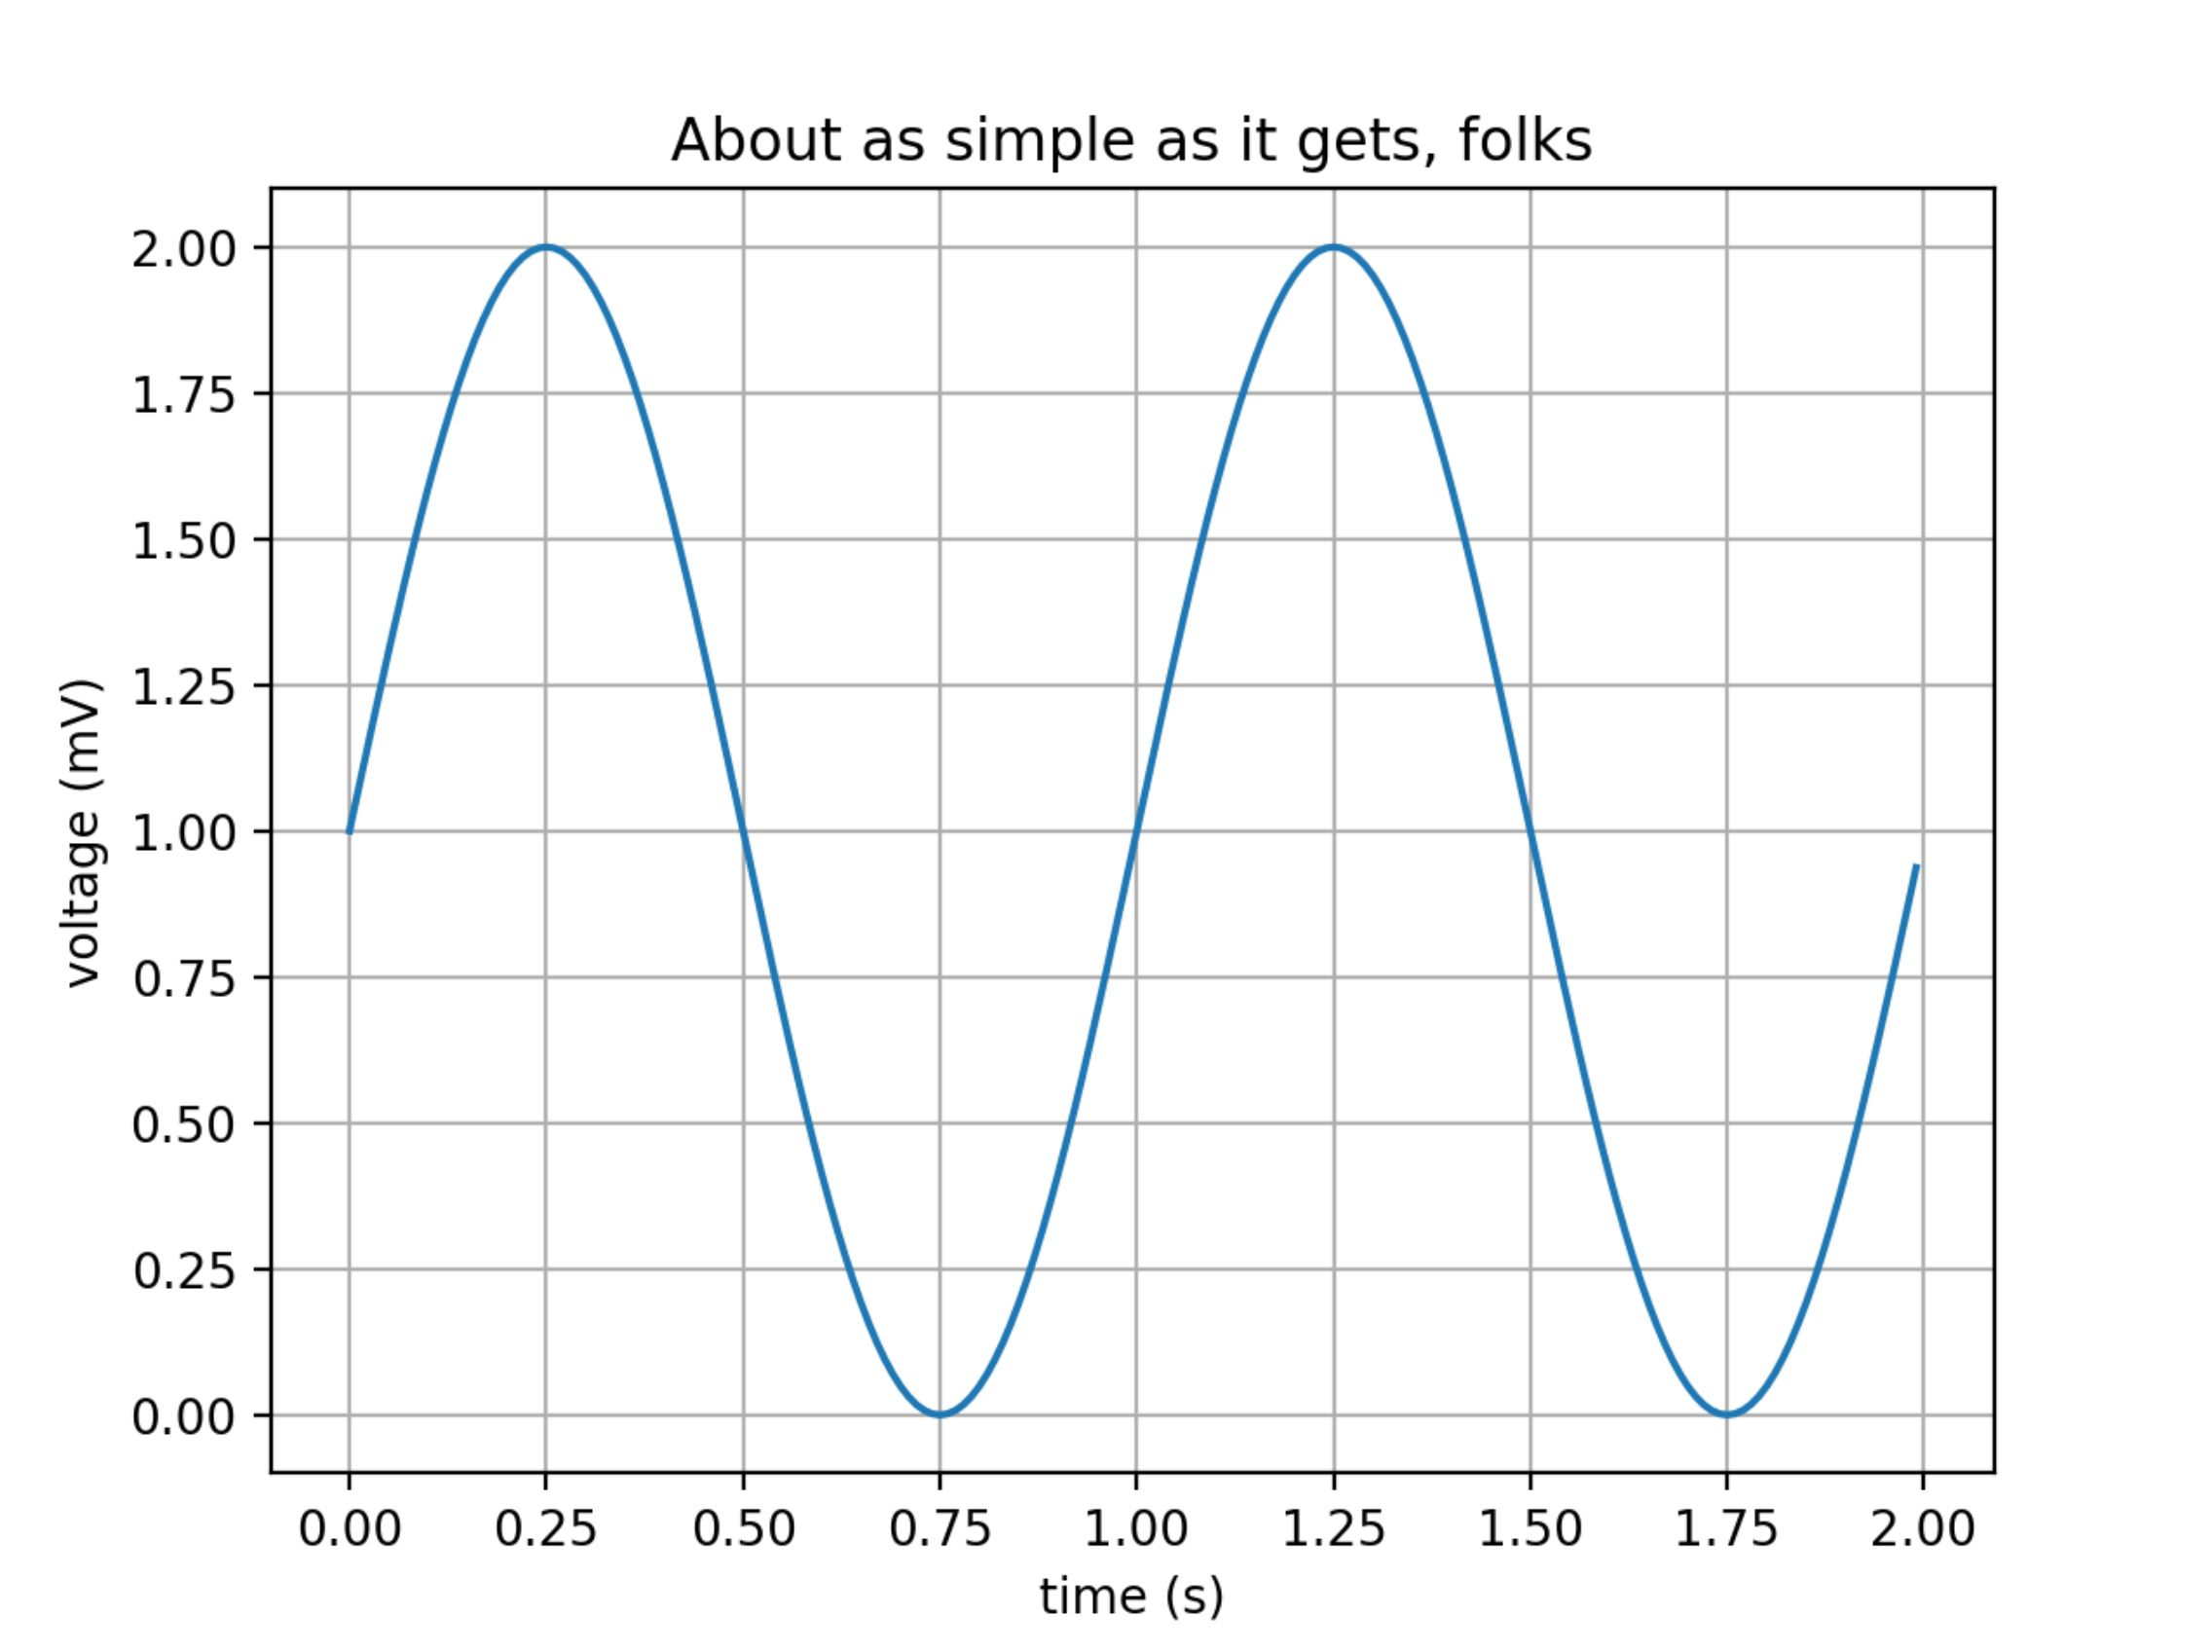
\includegraphics[width = 0.6\textwidth]{example1.png}
%    \caption{Test Figure}
%\end{figure}

%\clearpage
%\subsection{常用命令展示}
%这部分将展示其他常用命令。
%
%\begin{tbox}{颜色设置}
%\begin{itemize}
%	\item  \textcolor{Red}{赤}\textcolor{Orange}{橙}\textcolor{Yellow}{黄}\textcolor{Green}{绿}\textcolor{Emerald}{青}\textcolor{Blue}{蓝}\textcolor{Purple}{紫}
%	\item  谁持彩练当空舞
%\end{itemize}
%\end{tbox}
%
%\begin{tbox}{字号设置}
%\begin{enumerate}
%	\item {\LARGE 江晚正愁余}
%	\item {\Large 江晚正愁余}
%	\item {\large 江晚正愁余}
%	\item {\normalsize 江晚正愁余}
%	\item {\small 江晚正愁余}
%	\item {\footnotesize 江晚正愁余}
%	\item {\scriptsize 江晚正愁余}
%\end{enumerate}
%\end{tbox}
%
%\begin{tbox}{字体设置(中文)}
%\begin{enumerate}
%	\item 宋体:{\songti 山有扶苏,隰有荷华}
%	\item 仿宋:{\fangsong 山有扶苏,隰有荷华}
%	\item 黑体:{\heiti 山有扶苏,隰有荷华}
%	\item 楷书:{\kaishu 山有扶苏,隰有荷华}
%\end{enumerate}
%\end{tbox}
%
%\begin{tbox}{Set font(English)}
%\begin{enumerate}
%	\item roman:\quad{\rmfamily Hello world!}
%	\item sans-serif:\quad{\sffamily Hello world!}
%	\item typewriter:\quad{\ttfamily Hello world!}
%\end{enumerate}
%\end{tbox}
%
%\begin{tbox}{公式}
%	无编号公式
%    \begin{equation*}
%        J(\theta) = \mathbb{E}_{\pi_\theta}[G_t] = \sum_{s\in\mathcal{S}} d^\pi (s)V^\pi(s)=\sum_{s\in\mathcal{S}} d^\pi(s)\sum_{a\in\mathcal{A}}\pi_\theta(a|s)Q^\pi(s,a)
%    \end{equation*}
%$$ J(\theta) = \mathbb{E}_{\pi_\theta}[G_t] = \sum_{s\in\mathcal{S}} d^\pi (s)V^\pi(s)=\sum_{s\in\mathcal{S}} d^\pi(s)\sum_{a\in\mathcal{A}}\pi_\theta(a|s)Q^\pi(s,a) $$
%    有编号公式
%    \begin{equation}
%        J(\theta) = \mathbb{E}_{\pi_\theta}[G_t] = \sum_{s\in\mathcal{S}} d^\pi (s)V^\pi(s)=\sum_{s\in\mathcal{S}} d^\pi(s)\sum_{a\in\mathcal{A}}\pi_\theta(a|s)Q^\pi(s,a)
%    \end{equation}
%    \begin{equation}
%        J(\theta) = \mathbb{E}_{\pi_\theta}[G_t] = \sum_{s\in\mathcal{S}} d^\pi (s)V^\pi(s)=\sum_{s\in\mathcal{S}} d^\pi(s)\sum_{a\in\mathcal{A}}\pi_\theta(a|s)Q^\pi(s,a)
%    \end{equation}
%	波尔文积分
%    \[
%    \begin{cases}
%        \vspace{0.2cm}
%        \displaystyle{\int_{0}^{\infty} \frac{\sin(x)}{x}\,dx = \frac{\pi}{2}}\\
%        \vspace{0.2cm}
%        \displaystyle{\int_{0}^{\infty} \frac{\sin(x)}{x} \frac{\sin(x/3)}{x/3}\,dx = \frac{\pi}{2}} \\
%        \vspace{0.2cm}\cdot\cdot\cdot\\
%        \vspace{0.2cm}
%        \displaystyle{\int_{0}^{\infty} \frac{\sin(x)}{x} \frac{\sin(x/3)}{x/3} \cdot\cdot\cdot \frac{\sin(x/13)}{x/13}\,dx = \frac{\pi}{2}}\\
%        \displaystyle{\int_{0}^{\infty} \frac{\sin(x)}{x} \frac{\sin(x/3)}{x/3} \cdot\cdot\cdot \frac{\sin(x/15)}{x/15}\,dx = \frac{467807924713440738696537864469}{935615849440640907310521750000}\pi}
%    \end{cases}  
%    \]
%	多行对齐公式
%\begin{align*}
%    \frac{\partial}{\partial \theta_k}J(\theta) 
%        &= \frac{\partial}{\partial \theta_k}\Bigg[\frac{1}{m}\sum_{k=1}^m log(1+e^{-y^{(i)}\theta^Tx^{(i)}})\Bigg] \\
%        &= \frac{1}{m}\sum_{k=1}^m \frac{1}{1+e^{-y^{(i)}\theta^Tx^{(i)}}}y^{(i)}x_k^{(i)} \\
%        &= -\frac{1}{m}\sum_{k=1}^m h_\theta(-y^{(i)}x^{(i)})y^{(i)}x_k^{(i)}        
%\end{align*}
%\end{tbox}

%\begin{tbox}{引用}
%	对公式的引用,如\cref{equ:test}
%	\begin{equation}
%        J(\theta) = \mathbb{E}_{\pi_\theta}[G_t] = \sum_{s\in\mathcal{S}} d^\pi (s)V^\pi(s)=\sum_{s\in\mathcal{S}} d^\pi(s)\sum_{a\in\mathcal{A}}\pi_\theta(a|s)Q^\pi(s,a)
%		\label{equ:test}
%    \end{equation}
%	对图像的引用,如\cref{fig:test}
%	\begin{figure}[H]
%		\centering
%		
\includegraphics[width=0.3\textwidth]{example.png}
%		\caption{测试图片}
%		\label{fig:test}
%	\end{figure}
%	对表格的引用,如\cref{tab:test}
%	\begin{table}[H]
%		\renewcommand\arraystretch{1.5}
%		\caption{一个空表格}
%		\begin{tabularx}{\textwidth}{|p{0.15\textwidth}|X|X|X|X|}
%		\hline
%		 &  &  &  &  \\    
%		\hline
%		 &  &  & &  \\    
%		\hline
%		\end{tabularx}
%		\label{tab:test}
%	\end{table}
%\end{tbox}
%
%\begin{tbox}{表格}
%	tabular可以自己更改宽度
%	\begin{table}[H]
%		\renewcommand\arraystretch{1.7}
%		\centering
%		\caption{一个空表格}
%		\begin{tabular}{|p{0.15\textwidth}|p{0.15\textwidth}|p{0.15\textwidth}|p{0.15\textwidth}|}
%		\hline
%		&   &  &  \\
%		\hline
%		 &   &  &  \\
%		\hline    
%		\end{tabular}
%	\end{table}
%	tabularx可以自适应宽度
%	\begin{table}[H]
%		\renewcommand\arraystretch{1.7}
%		\centering
%		\caption{一个空表格}
%		\begin{tabularx}{\textwidth}{|p{0.2\textwidth}|X|X|X|X|X|X|}
%			\hline
%			& &  &  &  &  &  \\
%			\hline
%			 & &  &  &  &  &  \\
%			\hline
%		\end{tabularx}
%	\end{table}
%\end{tbox}
\end{document}
